%%%%%%%%%%%%%%%%%%%%%%%%%%%%%%%%%%%%%%%%%%%%%%%%%%%%%%%%%%%%%%%%%%%%%%%%%%%

\documentclass{standalone}

\usepackage{mathptmx}
\usepackage{tikz}
\usetikzlibrary{external}
\tikzexternalize{unit-triangle}

%% We default to Times.
\renewcommand{\rmdefault}{ptm}
\renewcommand{\ttdefault}{pcr}
%% Enable Times/Palatino main text font.
\normalfont\selectfont

\newcommand{\comma}{,\,}
\newcommand{\tuple}[2]{(#1\comma #2)}

%% The Cartesian coordinate system.
\newcommand{\cartesianCoordinate}{%%
  %% The x-axis.
  \draw[axisStyle] (xstart) -- (xend);
  \node at (xend) [right] {$x$};
  %% The y-axis.
  \draw[axisStyle] (ystart) -- (yend);
  \node at (yend) [above] {$y$};
}

%% A unit triangle.
\newcommand{\unitTriangle}{%%
  %% The sides of the unit triangle.
  \draw[lineStyle] (A) -- (B) -- (C);
  %% The corner points of the unit triangle.
  \xyPoint{A}{\tuple{\frac{1}{2}}{0}}{below}
  \xyPoint{B}{\tuple{0}{\frac{\sqrt{3}}{2}}}{above right}
  \xyPoint{C}{\tuple{-\frac{1}{2}}{0}}{below}
}

%% A point on the Cartesian plane.
%%
%% #1 -- The x- and y-coordinates of the point.
%% #2 -- Label the point with this name.
%% #3 -- Where to place the label relative to the point.
\newcommand{\xyPoint}[3]{%%
  \node[nodeStyle] at (#1) {};
  \node at (#1) [#3] {$#2$};
}

%% The three corners of a unit triangle.

\begin{document}

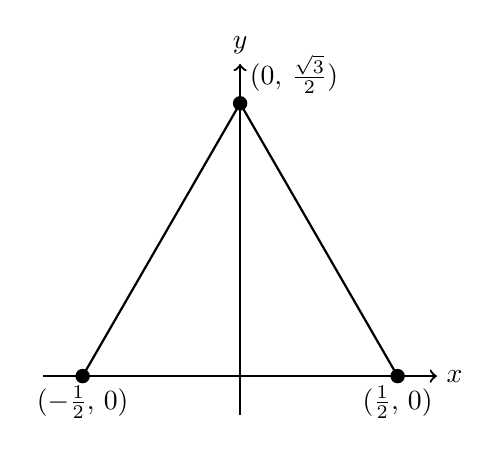
\begin{tikzpicture}[%%
  axisStyle/.style={->,thick},%%
  lineStyle/.style={-,thick},%%
  nodeStyle/.style={draw,inner sep=1.7pt,circle,fill=black,black}%%
]
%%
%%
%% Coordinates of the corner points.
\pgfmathsetmacro{\scaleFactor}{4}
\pgfmathsetmacro{\xa}{0.5*\scaleFactor}
\pgfmathsetmacro{\ya}{0*\scaleFactor}
\pgfmathsetmacro{\xb}{0*\scaleFactor}
\pgfmathsetmacro{\yb}{0.866025403784439*\scaleFactor}  %% \sqrt{3} / 2
\pgfmathsetmacro{\xc}{-0.5*\scaleFactor}
\pgfmathsetmacro{\yc}{0*\scaleFactor}
\coordinate (A) at (\xa,\ya);
\coordinate (B) at (\xb,\yb);
\coordinate (C) at (\xc,\yc);
%%
%% Coordinates of the minimum and maximum of the axes.
\pgfmathsetmacro{\dx}{0.5}
\pgfmathsetmacro{\xhigh}{\xa+\dx}
\pgfmathsetmacro{\xlow}{-\xa-\dx}
\pgfmathsetmacro{\yhigh}{\yb+\dx}
\pgfmathsetmacro{\ylow}{-0.5}
\coordinate (xend) at (\xhigh,0);
\coordinate (xstart) at (\xlow,0);
\coordinate (yend) at (0,\yhigh);
\coordinate (ystart) at (0,\ylow);
%%
%%
%% Illustrate a circle.
\cartesianCoordinate
\unitTriangle
\end{tikzpicture}

\end{document}
